\section{}
Suppose that a star is made of ideal gas, is dominated by radiative heat transfer, and is in hydrostatic equilibrium. Furthermore, the specific (per unit mass) energy generation, mean molecular weight, and opacity are the same throughout this star.
Neglecting radiation pressure, please show that the star is a polytrope of index $n = 3$.

\section{}
\textbf{Use some decent integrator to construct a polytrope with index $n = 3$.
The simplest method is to shoot for a solution. 
Please a) plot $\theta_3$ as a function of $\xi$ and b) calculate $\xi_1$, $-\theta_3^\prime(\xi_1)$, and $\rho_c/\langle\rho\rangle$ and check your results with Table 7.1 in HSK.}

To find a solution we start with Lane-Emden Equation given by 
\begin{equation}
    \frac{1}{\xi^2}\frac{d}{d\xi}\left(\xi^2\frac{d\theta_n}{d\xi}\right) = -\theta_n^n
\end{equation}
Following the textbook, we can do the substitutions $x=\xi$, $y=\theta_n$ and $z=y^\prime=dy/dx$, then Lane-Emden equation gets into
\begin{align*}
    \frac{1}{x^2}\frac{d}{dx}\left(x^2 z\right) = -y^n \\
    \frac{1}{x^2}(2xz + x^2z^\prime) =  -y^n \\
    z^\prime = -y^n - \frac{2z}{x} \numberthis \label{eq:LaneEmden}
\end{align*}

We can solve this equation for several values of n, including $n=3$. 

\begin{figure}
    \centering
    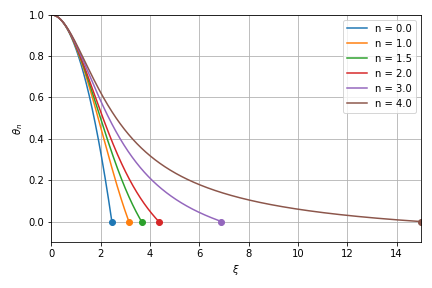
\includegraphics{CodeAndFigures/Astro643Hw3P2Plot.png}
    \caption{Solutions for polytropes with index values $n=0,1,1.5,2,3,4$ where the fill circles mark the position of $\xi_1$ defined by $\theta_n(\xi_1)=0$ and whose value can be seen on Table \ref{tab:LaneEmdenSolutions}.}
    \label{fig:LaneEmdenSolutions}
\end{figure}

\begin{table}[]
    \centering
    \begin{tabular}{rrrrrr}
\toprule
    n &  $\xi_1$ &  $\xi_1$ True &  $-\theta_n^\prime(\xi_1)$ &  $-\theta_n^\prime(\xi_1)$ True &  $\frac{1}{3}\left(\frac{\xi}{-\theta_n^\prime}\right)_{\xi_1}$ \\
\midrule
0.000 &    2.450 &         2.449 &                      0.817 &                           0.816 &                                              1.000 \\
1.000 &    3.142 &         3.142 &                      0.318 &                           0.318 &                                              3.291 \\
1.500 &    3.654 &         3.654 &                        NaN &                           0.203 &                                                NaN \\
2.000 &    4.353 &         4.353 &                      0.127 &                           0.127 &                                             11.404 \\
3.000 &    6.897 &         6.897 &                      0.042 &                           0.042 &                                             54.186 \\
4.000 &   14.972 &        14.972 &                      0.008 &                           0.008 &                                            622.465 \\
\bottomrule
\end{tabular}

    \caption{Solutions for polytropes with index values $n=0,1.5,1,2,3,4$ where the columns ending with "True" are the values given in Table 7.1 of the textbook and are included for comparison.}
    \label{tab:LaneEmdenSolutions}
\end{table}



\section{}
Estimate the Chandrasekhar's mass of a zero temperature white dwarf, when electrons become extreme relativistic degenerate.
\subsection{}
Show that the equation of state can be expressed as $P=K\rho^{4/3}$ where
\begin{equation}
    K = \frac{1}{4}\left(\frac{8\pi}{3}\right)^{-1/3}\frac{hc}{(m_A\mu_e)^{4/3}}
\end{equation}
in which $\mu_e$ is the mean molecular weight of electrons.

\subsection{}
Show the mass of the white dwarf in this extreme is independent of the radius
R and can be expressed as
\begin{equation}
    M = \frac{1}{4\pi}\left(\frac{3}{2}\right)^{1/2}\left(\frac{hc}{Gm_A^{4/3}}\right)^{3/2}\frac{\xi_1^2\left(-\frac{d\theta_3}{d\xi}\right)_{\xi_1}}{\mu_e^2},
\end{equation}

where the values of $\xi_1$ and $\left(-\frac{d\theta_3}{d\xi}\right)_{\xi_1}$ can be obtained from Table 7.1.

\subsection{}
Finally, show $M=1.44M_\odot\left(\frac{2}{\mu_e}\right)^2$. What is the value of $\mu_e$ for a white dwarf with He, C, O... composition (i.e., $X\sim0)$)?



\section{}
Consider a (fully convective) solar composition ($\mu = 0.61, \mu_e = 1.17$) object at the
star/brown dwarf dividing line. The object can be modeled via a polytrope with
$n = 3/2$.

\subsection{}
Please obtain the central density and temperature as a function of the total
radius (R) and mass (M) of the object in solar units.

\subsection{}
Show how the central temperature depends on the stellar mass when the gas
thermal pressure equals to the electron degeneracy pressure.

\subsection{}
The minimum temperature required to fuse hydrogen is $T_{min}\sim\SI{4e6}{\kelvin}$. Let's
assume that for fusion to occur, the object can't be supported by degeneracy,
i.e., gas pressure must be more important than degeneracy pressure. 
With this condition, what is the transition mass between stars and brown dwarfs?


\section{}
Derive the following equation (see Eq. 7.141 of the textbook, HSK)
\begin{equation}
    T_{eff}\approx 2400(Z/0.02)^{4/51}\mu^{13/51}(M/M_\odot)^{7/51}(L/L_\odot)^{1/102}
\end{equation}
for a completely convective star with $H^{-}$ opacity near the surface (see Eq. 7.126, HSK).



